\documentclass{article}\usepackage[]{graphicx}\usepackage[]{color}
%% maxwidth is the original width if it is less than linewidth
%% otherwise use linewidth (to make sure the graphics do not exceed the margin)
\makeatletter
\def\maxwidth{ %
  \ifdim\Gin@nat@width>\linewidth
    \linewidth
  \else
    \Gin@nat@width
  \fi
}
\makeatother

\definecolor{fgcolor}{rgb}{0.345, 0.345, 0.345}
\newcommand{\hlnum}[1]{\textcolor[rgb]{0.686,0.059,0.569}{#1}}%
\newcommand{\hlstr}[1]{\textcolor[rgb]{0.192,0.494,0.8}{#1}}%
\newcommand{\hlcom}[1]{\textcolor[rgb]{0.678,0.584,0.686}{\textit{#1}}}%
\newcommand{\hlopt}[1]{\textcolor[rgb]{0,0,0}{#1}}%
\newcommand{\hlstd}[1]{\textcolor[rgb]{0.345,0.345,0.345}{#1}}%
\newcommand{\hlkwa}[1]{\textcolor[rgb]{0.161,0.373,0.58}{\textbf{#1}}}%
\newcommand{\hlkwb}[1]{\textcolor[rgb]{0.69,0.353,0.396}{#1}}%
\newcommand{\hlkwc}[1]{\textcolor[rgb]{0.333,0.667,0.333}{#1}}%
\newcommand{\hlkwd}[1]{\textcolor[rgb]{0.737,0.353,0.396}{\textbf{#1}}}%
\let\hlipl\hlkwb

\usepackage{framed}
\makeatletter
\newenvironment{kframe}{%
 \def\at@end@of@kframe{}%
 \ifinner\ifhmode%
  \def\at@end@of@kframe{\end{minipage}}%
  \begin{minipage}{\columnwidth}%
 \fi\fi%
 \def\FrameCommand##1{\hskip\@totalleftmargin \hskip-\fboxsep
 \colorbox{shadecolor}{##1}\hskip-\fboxsep
     % There is no \\@totalrightmargin, so:
     \hskip-\linewidth \hskip-\@totalleftmargin \hskip\columnwidth}%
 \MakeFramed {\advance\hsize-\width
   \@totalleftmargin\z@ \linewidth\hsize
   \@setminipage}}%
 {\par\unskip\endMakeFramed%
 \at@end@of@kframe}
\makeatother

\definecolor{shadecolor}{rgb}{.97, .97, .97}
\definecolor{messagecolor}{rgb}{0, 0, 0}
\definecolor{warningcolor}{rgb}{1, 0, 1}
\definecolor{errorcolor}{rgb}{1, 0, 0}
\newenvironment{knitrout}{}{} % an empty environment to be redefined in TeX

\usepackage{alltt}

\usepackage{fancyhdr} % Required for custom headers
\usepackage{lastpage} % Required to determine the last page for the footer
\usepackage{extramarks} % Required for headers and footers
\usepackage{graphicx} % Required to insert images
\usepackage{hyperref}
\usepackage{amsmath} %for binomial pdf
\usepackage{parskip} % so that there's space bw paragraphs
\usepackage{float}
\usepackage{amsfonts}

% Margins
\topmargin=-0.45in
\evensidemargin=0in
\oddsidemargin=0in
\textwidth=6.5in
\textheight=9.0in
\headsep=0.25in 

\linespread{1.1} % Line spacing

% Set up the header and footer
\pagestyle{fancy}
\lhead{STAT 534: Spatial} % Top left header
\chead{HW 7} % Top center header
\rhead{Andrea Mack} % Top right header
\lfoot{03/06/2017} % Bottom left footer
\cfoot{} % Bottom center footer
\rfoot{Page\ \thepage\ of\ \pageref{LastPage}} % Bottom right footer
\renewcommand\headrulewidth{0.4pt} % Size of the header rule
\renewcommand\footrulewidth{0.4pt} % Size of the footer rule

\setlength\parindent{0pt} % Removes all indentation from paragraphs
\setlength\parskip{0.5cm}
\restylefloat{table}

%----------------------------------------------------------------------------------------
%	DOCUMENT STRUCTURE COMMANDS
%	Skip this unless you know what you're doing
%----------------------------------------------------------------------------------------

% Header and footer for when a page split occurs within a problem environment
\newcommand{\enterProblemHeader}[1]{
\nobreak\extramarks{#1}{#1 continued on next page\ldots}\nobreak
\nobreak\extramarks{#1 (continued)}{#1 continued on next page\ldots}\nobreak
}

% Header and footer for when a page split occurs between problem environments
\newcommand{\exitProblemHeader}[1]{
\nobreak\extramarks{#1 (continued)}{#1 continued on next page\ldots}\nobreak
\nobreak\extramarks{#1}{}\nobreak
}


%----------------------------------------------------------------------------------------%
\IfFileExists{upquote.sty}{\usepackage{upquote}}{}
\begin{document}



\begin{enumerate}
\item %1
{\it A data set (wheat.txt) has been sent to you. The data set contains yields of wheat recorded at spatial coordinates. Note that the header is x, y, and z with z being the yields. We will need a couple of different data object types. Pay attention to the R code below. Do not worry about anisotropy.}

\begin{knitrout}\footnotesize
\definecolor{shadecolor}{rgb}{0.969, 0.969, 0.969}\color{fgcolor}\begin{kframe}
\begin{alltt}
\hlstd{wt} \hlkwb{<-} \hlkwd{read.table}\hlstd{(}\hlstr{"wheat.txt"}\hlstd{,} \hlkwc{header} \hlstd{=} \hlnum{TRUE}\hlstd{)}
\hlkwd{require}\hlstd{(geoR)}
\hlkwd{head}\hlstd{(wt)}
\end{alltt}
\begin{verbatim}
    x    y     z
1 4.3 19.2 29.25
2 4.3 20.4 31.55
3 4.3 21.6 35.05
4 4.3 22.8 30.10
5 4.3 24.0 33.05
6 4.3 25.2 30.25
\end{verbatim}
\begin{alltt}
\hlkwd{summary}\hlstd{(wt)}
\end{alltt}
\begin{verbatim}
       x               y               z        
 Min.   : 4.30   Min.   : 1.20   Min.   : 1.05  
 1st Qu.:17.20   1st Qu.: 7.20   1st Qu.:23.52  
 Median :25.80   Median :14.40   Median :26.85  
 Mean   :27.22   Mean   :14.08   Mean   :25.53  
 3rd Qu.:38.70   3rd Qu.:20.40   3rd Qu.:30.39  
 Max.   :47.30   Max.   :26.40   Max.   :42.00  
\end{verbatim}
\begin{alltt}
\hlkwd{str}\hlstd{(wt)}
\end{alltt}
\begin{verbatim}
'data.frame':	224 obs. of  3 variables:
 $ x: num  4.3 4.3 4.3 4.3 4.3 4.3 4.3 8.6 8.6 8.6 ...
 $ y: num  19.2 20.4 21.6 22.8 24 25.2 26.4 1.2 2.4 3.6 ...
 $ z: num  29.2 31.6 35 30.1 33 ...
\end{verbatim}
\begin{alltt}
\hlstd{wt} \hlkwb{<-} \hlkwd{data.frame}\hlstd{(}\hlkwd{apply}\hlstd{(wt,}\hlnum{2}\hlstd{,}\hlkwa{function}\hlstd{(}\hlkwc{t}\hlstd{)\{}
  \hlkwd{as.numeric}\hlstd{(}\hlkwd{as.character}\hlstd{(t))}
\hlstd{\}))}

\hlstd{wheat.dat} \hlkwb{<-} \hlstd{wt}
\hlstd{wheat.geodat} \hlkwb{<-} \hlkwd{as.geodata}\hlstd{(wheat.dat,} \hlkwc{coords.col}\hlstd{=}\hlnum{1}\hlopt{:}\hlnum{2}\hlstd{,}\hlkwc{data.col}\hlstd{=}\hlnum{3}\hlstd{)}

\hlcom{# warnings for eliminating rows with NAs}

\hlstd{wheat.grid} \hlkwb{<-} \hlkwd{expand.grid}\hlstd{(}\hlkwd{seq}\hlstd{(}\hlnum{0}\hlstd{,}\hlnum{50}\hlstd{,}\hlkwc{l}\hlstd{=}\hlnum{25}\hlstd{),}
                           \hlkwd{seq}\hlstd{(}\hlnum{0}\hlstd{,}\hlnum{30}\hlstd{,}\hlkwc{l}\hlstd{=}\hlnum{25}\hlstd{))}
\end{alltt}
\end{kframe}
\end{knitrout}

\begin{enumerate}
\item%1a
{\it Plot the data and comment on the results.}

There appears to be a trend in both the east-west and north-south directions. The data are skewed left. Quantiles associated with the blue color are clustered mostly at high X coordinate values and low Y coordinate values.

\begin{knitrout}\footnotesize
\definecolor{shadecolor}{rgb}{0.969, 0.969, 0.969}\color{fgcolor}\begin{kframe}
\begin{alltt}
\hlkwd{plot}\hlstd{(wheat.geodat)}
\end{alltt}
\end{kframe}

{\centering 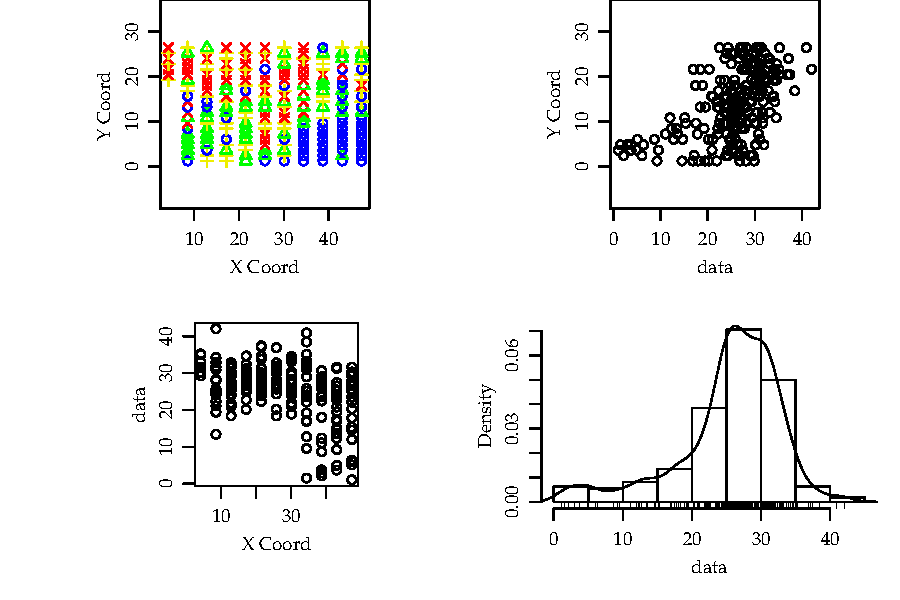
\includegraphics[width=\maxwidth]{figure/prob1a-1} 

}



\end{knitrout}

\item 
{\it Produce a plot of the empirical semivariogram of the wheat yields. Can this plot be trusted for estimation of semivariogram parameters to be used in kriging. Why or why not?}

In the presence of a trend, which we saw in (a), the empirical semivariogram estimator is biased.
\begin{knitrout}\footnotesize
\definecolor{shadecolor}{rgb}{0.969, 0.969, 0.969}\color{fgcolor}\begin{kframe}
\begin{alltt}
\hlstd{wheat.variog} \hlkwb{<-} \hlkwd{variog}\hlstd{(wheat.geodat,} \hlkwc{max.dist} \hlstd{=} \hlkwd{max}\hlstd{(}\hlkwd{dist}\hlstd{(wheat.geodat}\hlopt{$}\hlstd{coords)),}
                    \hlkwc{uvec} \hlstd{=} \hlnum{30}\hlstd{,} \hlkwc{messages} \hlstd{=} \hlnum{FALSE}\hlstd{)}

\hlkwd{plot}\hlstd{(wheat.variog,} \hlkwc{main} \hlstd{=} \hlstr{"Empirical Semivariogram"}\hlstd{)}
\end{alltt}
\end{kframe}

{\centering 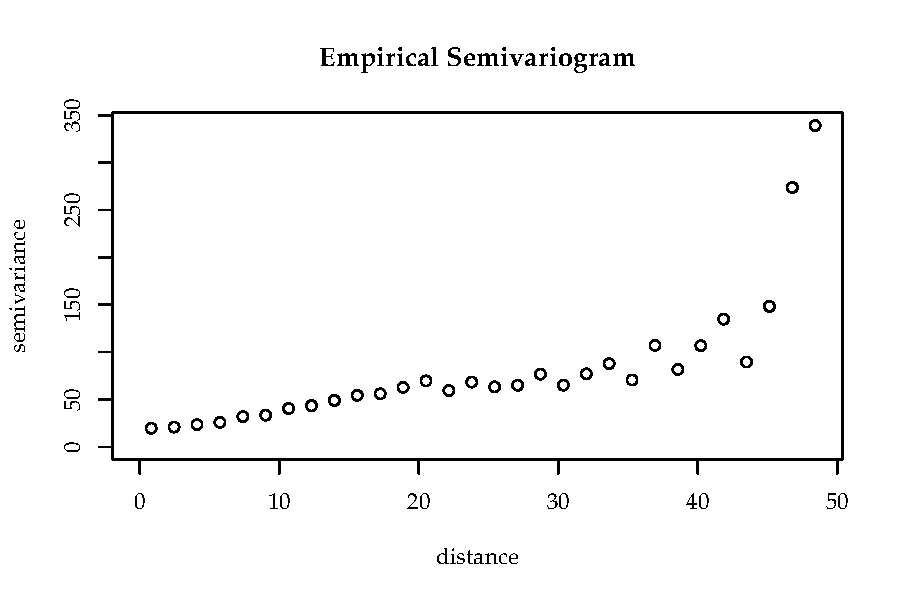
\includegraphics[width=\maxwidth]{figure/prob1b-1} 

}



\end{knitrout}

\item
{\it We will use the surf.ls function in the spatial library to fit a quadratic trend model to the yields by ordinary least squares and plot the empirical semivariogram of the residuals. Fit an appropriate semivariogram model to the semivariogram using your method of choice. Justify your final selection.}

I used the REML method because theoretically it provides valid standard errors if the assumptions are met (p. 24) and REML ensures positive variance estimates. I used initial covariance parameters estimated ``by eye" from the empirical semi-variogram.

I considered all the exponential, spherical, and gaussian models. The final model I will choose is the spherical model because the corresponding estimates are much more reasonable than either the exponential or gaussian model estimates.

%The initial plot shows fewer points on the edges of the east-west directions than in the center of the east-west directions. However, there does not appear to be any unusual points and so I will choose the ``classical" method of estimation, although both are plotted below.

\begin{knitrout}\footnotesize
\definecolor{shadecolor}{rgb}{0.969, 0.969, 0.969}\color{fgcolor}\begin{kframe}
\begin{alltt}
\hlkwd{require}\hlstd{(spatial)}
\hlstd{wheat.ls}\hlkwb{<-}\hlkwd{surf.ls}\hlstd{(}\hlnum{2}\hlstd{,wheat.dat)} \hlcom{# fits a second order polynomial trend surface}
\hlstd{resid.dat}\hlkwb{<-}\hlkwd{cbind}\hlstd{(wheat.dat}\hlopt{$}\hlstd{x,wheat.dat}\hlopt{$}\hlstd{y,}\hlkwd{residuals}\hlstd{(wheat.ls))}
\hlstd{resid.geodat}\hlkwb{<-}\hlkwd{as.geodata}\hlstd{(resid.dat,}\hlkwc{coords.col}\hlstd{=}\hlnum{1}\hlopt{:}\hlnum{2}\hlstd{,}\hlkwc{data.col}\hlstd{=}\hlnum{3}\hlstd{)}

\hlkwd{plot}\hlstd{(resid.geodat)}
\end{alltt}
\end{kframe}

{\centering 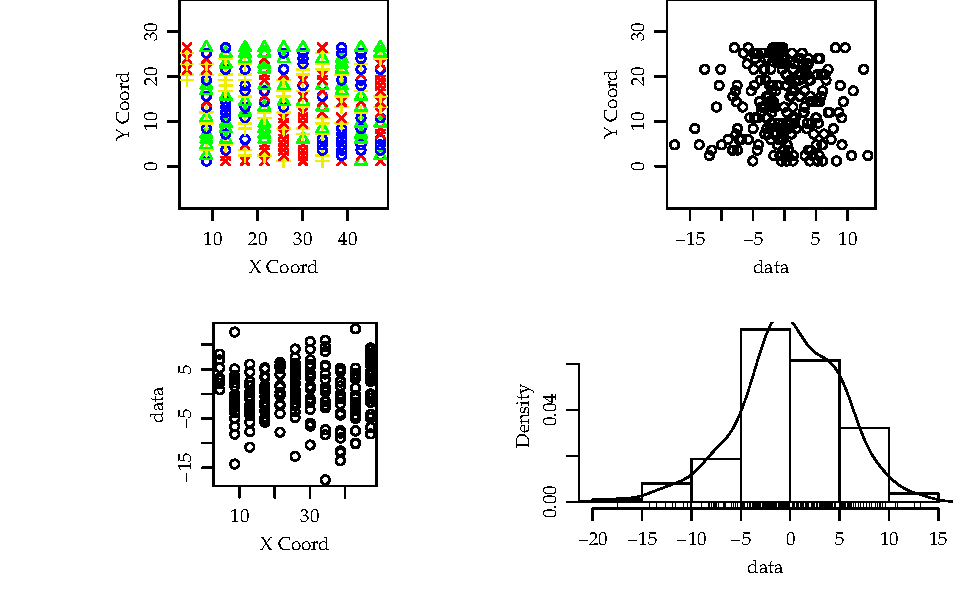
\includegraphics[width=\maxwidth]{figure/prob1c-1} 

}


\begin{kframe}\begin{alltt}
\hlkwd{par}\hlstd{(}\hlkwc{mfrow}\hlstd{=}\hlkwd{c}\hlstd{(}\hlnum{1}\hlstd{,}\hlnum{2}\hlstd{))}

\hlcom{#no outliers, use classical}
\hlstd{resid.class} \hlkwb{<-} \hlkwd{variog}\hlstd{(resid.geodat,} \hlkwc{coords} \hlstd{= resid.geodat}\hlopt{$}\hlstd{coords,} \hlkwc{data} \hlstd{= resid.geodat}\hlopt{$}\hlstd{data,} \hlkwc{uvec} \hlstd{=} \hlnum{30}\hlstd{,}
            \hlkwc{estimator.type} \hlstd{=} \hlstr{"classical"}\hlstd{,} \hlkwc{messages} \hlstd{=} \hlnum{FALSE}\hlstd{)}
\hlkwd{plot}\hlstd{(resid.class)}
\hlcom{#not attaining sill}

\hlcom{#cov.pars=(partialsill= 42-20, phi = 50)}
\hlcom{#cov.model = "exponential"}
\hlcom{#fix.nugget = TRUE -- it is quite stable?}
\hlcom{#nugget = 20}

\hlstd{exp.ml} \hlkwb{<-} \hlkwd{likfit}\hlstd{(resid.geodat,} \hlkwc{ini}\hlstd{=}\hlkwd{c}\hlstd{(}\hlnum{22}\hlstd{,}\hlnum{50}\hlopt{/}\hlnum{3}\hlstd{),} \hlkwc{fix.nugget} \hlstd{=} \hlnum{TRUE}\hlstd{,} \hlkwc{nugget} \hlstd{=} \hlnum{20}\hlstd{,}
                 \hlkwc{cov.model} \hlstd{=} \hlstr{"exponential"}\hlstd{)}
\end{alltt}
\begin{verbatim}
kappa not used for the exponential correlation function
---------------------------------------------------------------
likfit: likelihood maximisation using the function optim.
likfit: Use control() to pass additional
         arguments for the maximisation function.
        For further details see documentation for optim.
likfit: It is highly advisable to run this function several
        times with different initial values for the parameters.
likfit: WARNING: This step can be time demanding!
---------------------------------------------------------------
likfit: end of numerical maximisation.
\end{verbatim}
\begin{alltt}
\hlstd{exp.reml} \hlkwb{<-} \hlkwd{likfit}\hlstd{(resid.geodat,} \hlkwc{ini}\hlstd{=}\hlkwd{c}\hlstd{(}\hlnum{22}\hlstd{,}\hlnum{50}\hlopt{/}\hlnum{3}\hlstd{),} \hlkwc{fix.nugget} \hlstd{=} \hlnum{TRUE}\hlstd{,} \hlkwc{nugget} \hlstd{=} \hlnum{20}\hlstd{,}
                 \hlkwc{cov.model} \hlstd{=} \hlstr{"exponential"}\hlstd{,} \hlkwc{lik.method} \hlstd{=} \hlstr{"REML"}\hlstd{)}
\end{alltt}
\begin{verbatim}
kappa not used for the exponential correlation function
---------------------------------------------------------------
likfit: likelihood maximisation using the function optim.
likfit: Use control() to pass additional
         arguments for the maximisation function.
        For further details see documentation for optim.
likfit: It is highly advisable to run this function several
        times with different initial values for the parameters.
likfit: WARNING: This step can be time demanding!
---------------------------------------------------------------
likfit: end of numerical maximisation.
\end{verbatim}
\begin{alltt}
\hlstd{exp.ml}\hlopt{$}\hlstd{cov.pars}
\end{alltt}
\begin{verbatim}
[1] 8.313124 4.934723
\end{verbatim}
\begin{alltt}
\hlstd{exp.reml}\hlopt{$}\hlstd{cov.pars}
\end{alltt}
\begin{verbatim}
[1] 9.341821 5.935625
\end{verbatim}
\begin{alltt}
\hlstd{sph.ml} \hlkwb{<-} \hlkwd{likfit}\hlstd{(resid.geodat,} \hlkwc{ini}\hlstd{=}\hlkwd{c}\hlstd{(}\hlnum{22}\hlstd{,}\hlnum{50}\hlstd{),} \hlkwc{fix.nugget} \hlstd{=} \hlnum{TRUE}\hlstd{,} \hlkwc{nugget} \hlstd{=} \hlnum{20}\hlstd{,}
                 \hlkwc{cov.model} \hlstd{=} \hlstr{"sph"}\hlstd{,} \hlkwc{messages} \hlstd{=} \hlnum{FALSE}\hlstd{)}

\hlstd{sph.reml} \hlkwb{<-} \hlkwd{likfit}\hlstd{(resid.geodat,} \hlkwc{ini}\hlstd{=}\hlkwd{c}\hlstd{(}\hlnum{22}\hlstd{,}\hlnum{50}\hlstd{),} \hlkwc{fix.nugget} \hlstd{=} \hlnum{TRUE}\hlstd{,} \hlkwc{nugget} \hlstd{=} \hlnum{20}\hlstd{,}
                 \hlkwc{cov.model} \hlstd{=} \hlstr{"sph"}\hlstd{,} \hlkwc{lik.method} \hlstd{=} \hlstr{"REML"}\hlstd{,} \hlkwc{messages} \hlstd{=} \hlnum{FALSE}\hlstd{)}

\hlstd{sph.ml}\hlopt{$}\hlstd{cov.pars}
\end{alltt}
\begin{verbatim}
[1] 27.73756 42.79786
\end{verbatim}
\begin{alltt}
\hlstd{sph.reml}\hlopt{$}\hlstd{cov.pars}
\end{alltt}
\begin{verbatim}
[1] 30.04778 43.43237
\end{verbatim}
\begin{alltt}
\hlstd{gaus.ml} \hlkwb{<-} \hlkwd{likfit}\hlstd{(resid.geodat,} \hlkwc{ini}\hlstd{=}\hlkwd{c}\hlstd{(}\hlnum{22}\hlstd{,}\hlnum{50}\hlopt{/}\hlkwd{sqrt}\hlstd{(}\hlnum{3}\hlstd{)),} \hlkwc{fix.nugget} \hlstd{=} \hlnum{TRUE}\hlstd{,} \hlkwc{nugget} \hlstd{=} \hlnum{20}\hlstd{,}
                 \hlkwc{cov.model} \hlstd{=} \hlstr{"gau"}\hlstd{,} \hlkwc{messages} \hlstd{=} \hlnum{FALSE}\hlstd{)}
\hlstd{gaus.reml} \hlkwb{<-} \hlkwd{likfit}\hlstd{(resid.geodat,} \hlkwc{ini}\hlstd{=}\hlkwd{c}\hlstd{(}\hlnum{22}\hlstd{,}\hlnum{50}\hlopt{/}\hlkwd{sqrt}\hlstd{(}\hlnum{3}\hlstd{)),} \hlkwc{fix.nugget} \hlstd{=} \hlnum{TRUE}\hlstd{,} \hlkwc{nugget} \hlstd{=} \hlnum{20}\hlstd{,}
                 \hlkwc{cov.model} \hlstd{=} \hlstr{"gau"}\hlstd{,} \hlkwc{lik.method} \hlstd{=} \hlstr{"REML"}\hlstd{,} \hlkwc{messages} \hlstd{=} \hlnum{FALSE}\hlstd{)}

\hlstd{gaus.ml}\hlopt{$}\hlstd{cov.pars}
\end{alltt}
\begin{verbatim}
[1] 7.738056 6.079979
\end{verbatim}
\begin{alltt}
\hlstd{gaus.reml}\hlopt{$}\hlstd{cov.pars}
\end{alltt}
\begin{verbatim}
[1] 8.415170 6.315104
\end{verbatim}
\end{kframe}

{\centering 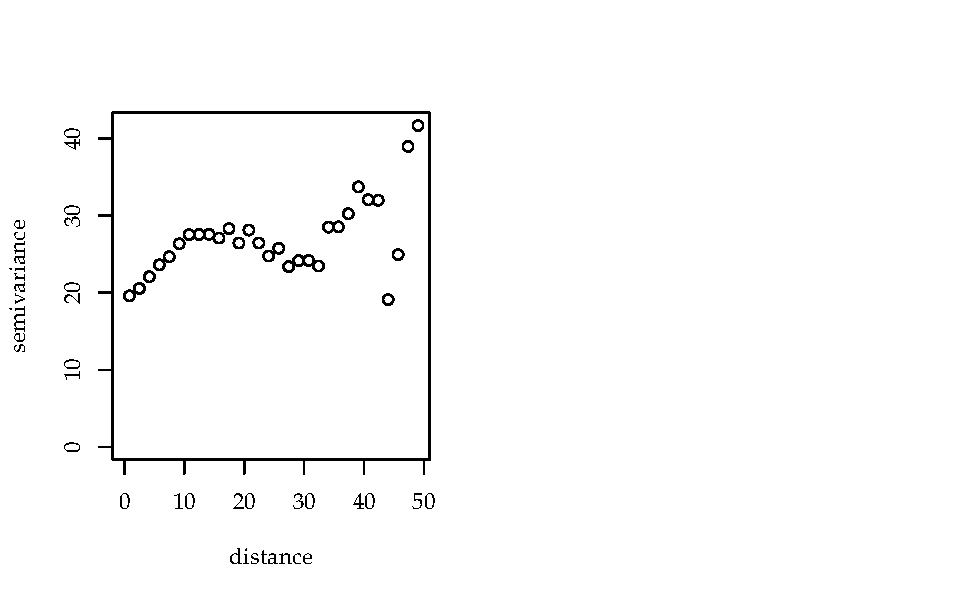
\includegraphics[width=\maxwidth]{figure/prob1c-2} 

}



\end{knitrout}

\item
{\it Predict yields using universal kriging and ordinary kriging. Use the parameter estimates from the residual semivariogram when you do ordinary kriging. Plot the results along with a plot of the kriging standard errors. Remember to be careful of that range parameter - what you enter depends on which semivariogram model you used. Compare the results and comment.}

{\bf Fit an OK model using the residual semivariogram parameter estimates and then fit a UK model using the same estimates.}

Both OK and UK results show similar rough-ness patterns in the prediction contour plot. The UK model produced more extreme predictions than the OK results. The prediction SE's are exactly the same.

\begin{knitrout}\footnotesize
\definecolor{shadecolor}{rgb}{0.969, 0.969, 0.969}\color{fgcolor}\begin{kframe}
\begin{alltt}
\hlcom{# Note trend=2,m0="kt" in the argument list when doing universal kriging.}
\hlstd{nugget} \hlkwb{<-} \hlstd{sph.reml}\hlopt{$}\hlstd{nugget}
\hlstd{effsill} \hlkwb{<-} \hlstd{sph.reml}\hlopt{$}\hlstd{cov.pars[}\hlnum{1}\hlstd{]} \hlopt{+} \hlstd{nugget}
\hlstd{range} \hlkwb{<-} \hlstd{sph.reml}\hlopt{$}\hlstd{cov.pars[}\hlnum{2}\hlstd{]}
\hlstd{wheat.uk}\hlkwb{<-}\hlkwd{ksline}\hlstd{(wheat.geodat,}\hlkwc{locations}\hlstd{=wheat.grid,}\hlkwc{cov.model}\hlstd{=}\hlstr{"spherical"}\hlstd{,}
\hlkwc{cov.pars}\hlstd{=}\hlkwd{c}\hlstd{(effsill,range),}
\hlkwc{nugget}\hlstd{=nugget,}\hlkwc{trend}\hlstd{=}\hlnum{2}\hlstd{,}\hlkwc{m0}\hlstd{=}\hlstr{"kt"}\hlstd{)}
\end{alltt}
\begin{verbatim}
ksline: kriging location:  1 out of 625 
ksline: kriging location:  101 out of 625 
ksline: kriging location:  201 out of 625 
ksline: kriging location:  301 out of 625 
ksline: kriging location:  401 out of 625 
ksline: kriging location:  501 out of 625 
ksline: kriging location:  601 out of 625 
ksline: kriging location:  625 out of 625 
Kriging performed using global neighbourhood 
\end{verbatim}
\begin{alltt}
\hlcom{#note hpts is not defined in the notes?}

\hlkwd{par}\hlstd{(}\hlkwc{mfrow}\hlstd{=}\hlkwd{c}\hlstd{(}\hlnum{1}\hlstd{,}\hlnum{1}\hlstd{))}
\hlstd{htps} \hlkwb{<-} \hlkwd{chull}\hlstd{(wheat.dat[,}\hlnum{1}\hlstd{],wheat.dat[,}\hlnum{2}\hlstd{])}
\hlstd{htps} \hlkwb{<-} \hlkwd{c}\hlstd{(htps,htps[}\hlnum{1}\hlstd{])}
\hlkwd{contour}\hlstd{(wheat.uk,}\hlkwc{nlevels}\hlstd{=}\hlnum{15}\hlstd{,} \hlkwc{main} \hlstd{=} \hlstr{"Universal Kriging"}\hlstd{)}
\hlkwd{lines}\hlstd{(wheat.dat[htps,}\hlnum{1}\hlstd{],wheat.dat[htps,}\hlnum{2}\hlstd{])}
\end{alltt}
\end{kframe}

{\centering 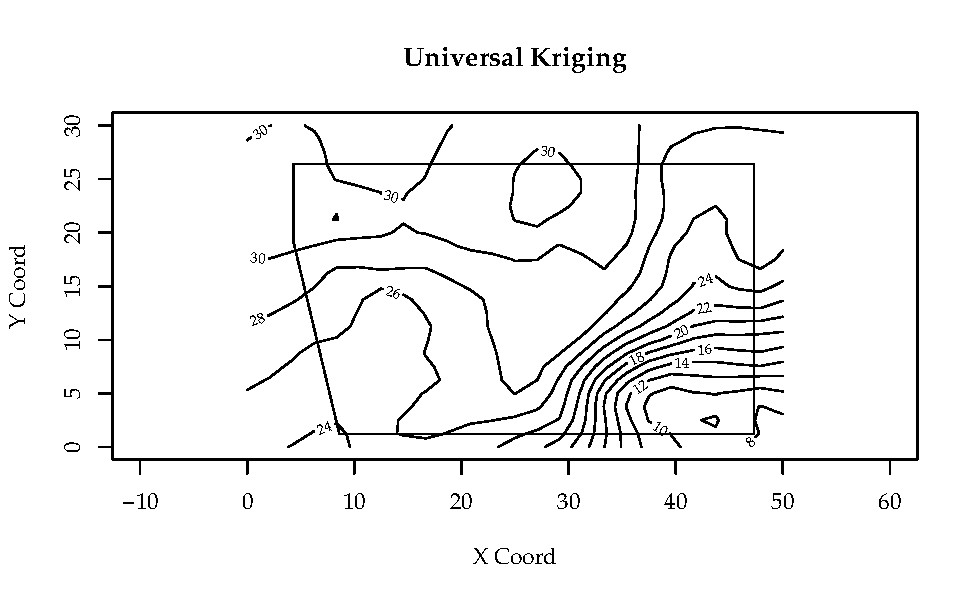
\includegraphics[width=\maxwidth]{figure/prob1d-1} 

}


\begin{kframe}\begin{alltt}
\hlstd{bord} \hlkwb{<-} \hlstd{wheat.dat[}\hlkwd{chull}\hlstd{(wheat.dat[,}\hlnum{1}\hlstd{],wheat.dat[,}\hlnum{2}\hlstd{]),}\hlopt{-}\hlkwd{c}\hlstd{(}\hlnum{3}\hlopt{:}\hlnum{5}\hlstd{)]}
\hlstd{pred.grid}\hlkwb{<-}\hlkwd{expand.grid}\hlstd{(}\hlkwd{seq}\hlstd{(}\hlopt{-}\hlnum{10}\hlstd{,}\hlnum{60}\hlstd{,}\hlkwc{l}\hlstd{=}\hlnum{30}\hlstd{),}\hlkwd{seq}\hlstd{(}\hlopt{-}\hlnum{10}\hlstd{,}\hlnum{60}\hlstd{,}\hlkwc{l}\hlstd{=}\hlnum{30}\hlstd{))}

\hlstd{kr.border} \hlkwb{<-} \hlkwd{ksline}\hlstd{(wheat.geodat,}\hlkwc{locations}\hlstd{=pred.grid,}
                    \hlkwc{borders}\hlstd{=bord,}
                    \hlkwc{cov.model} \hlstd{=} \hlstr{"spherical"}\hlstd{,} \hlkwc{cov.pars} \hlstd{=} \hlkwd{c}\hlstd{(}\hlnum{22}\hlstd{,}\hlnum{50}\hlstd{),}
                    \hlkwc{nugget} \hlstd{=} \hlnum{20}\hlstd{,}\hlkwc{m0}\hlstd{=}\hlstr{"kt"}\hlstd{,}\hlkwc{trend}\hlstd{=}\hlnum{1}\hlstd{,} \hlkwc{messages} \hlstd{=} \hlnum{FALSE}\hlstd{)}
\hlkwd{contour}\hlstd{(kr.border,}\hlkwc{val}\hlstd{=}\hlkwd{sqrt}\hlstd{(kr.border}\hlopt{$}\hlstd{krige.var))}
\hlkwd{title}\hlstd{(}\hlkwc{main}\hlstd{=}\hlstr{"Universal Kriging SEs"}\hlstd{)}
\end{alltt}
\end{kframe}

{\centering 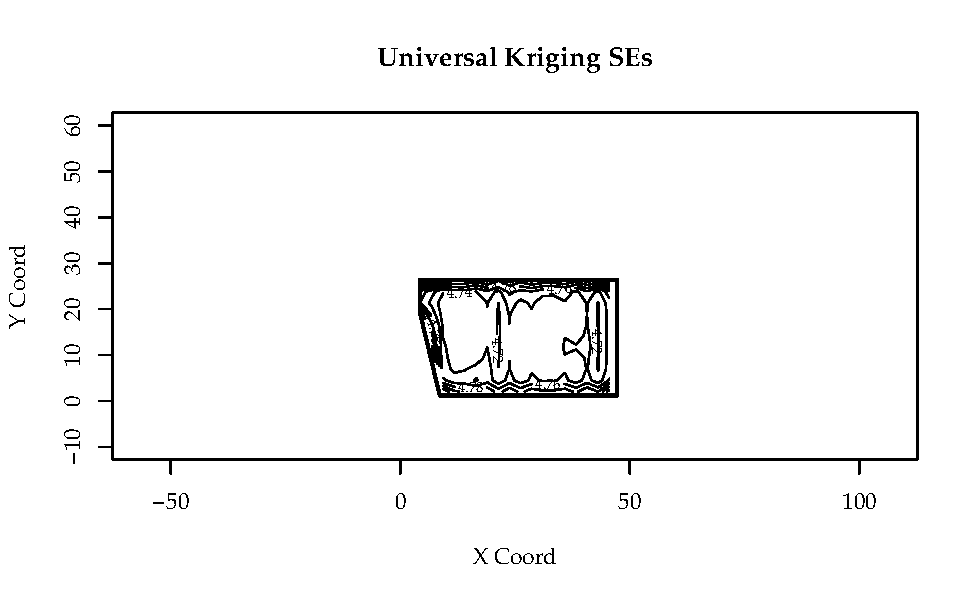
\includegraphics[width=\maxwidth]{figure/prob1d-2} 

}


\begin{kframe}\begin{alltt}
\hlstd{wheat.ok}\hlkwb{<-}\hlkwd{ksline}\hlstd{(wheat.geodat,}\hlkwc{locations}\hlstd{=wheat.grid,}\hlkwc{cov.model}\hlstd{=}\hlstr{"spherical"}\hlstd{,}
\hlkwc{cov.pars}\hlstd{=}\hlkwd{c}\hlstd{(effsill,range),}\hlkwc{nugget}\hlstd{=nugget)}
\end{alltt}
\begin{verbatim}
ksline: kriging location:  1 out of 625 
ksline: kriging location:  101 out of 625 
ksline: kriging location:  201 out of 625 
ksline: kriging location:  301 out of 625 
ksline: kriging location:  401 out of 625 
ksline: kriging location:  501 out of 625 
ksline: kriging location:  601 out of 625 
ksline: kriging location:  625 out of 625 
Kriging performed using global neighbourhood 
\end{verbatim}
\begin{alltt}
\hlkwd{contour}\hlstd{(wheat.ok,}\hlkwc{nlevels}\hlstd{=}\hlnum{15}\hlstd{,} \hlkwc{main} \hlstd{=}\hlstr{"Oridinary Kriging"}\hlstd{)}
\hlkwd{lines}\hlstd{(wheat.dat[htps,}\hlnum{1}\hlstd{],wheat.dat[htps,}\hlnum{2}\hlstd{])}
\end{alltt}
\end{kframe}

{\centering 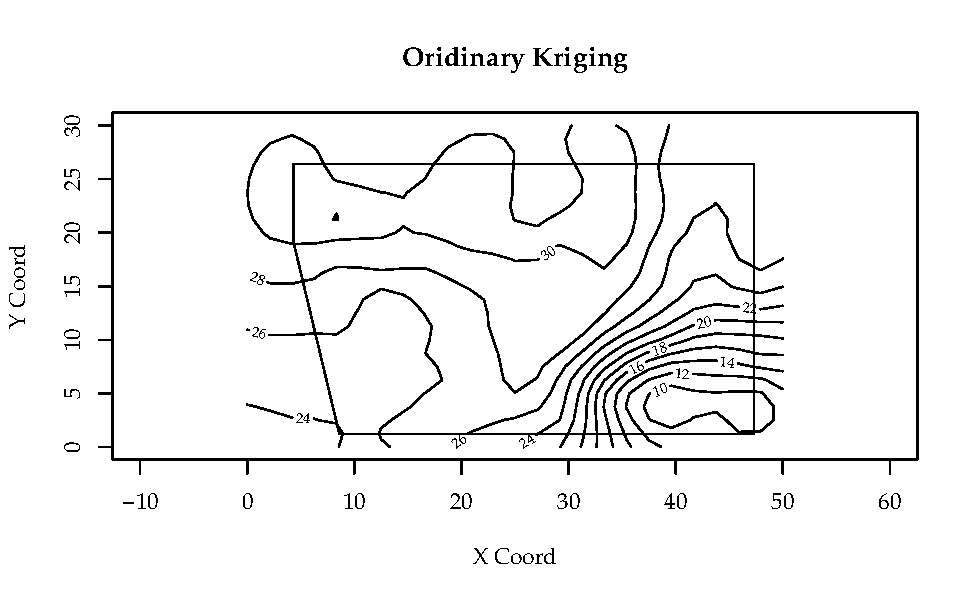
\includegraphics[width=\maxwidth]{figure/prob1d-3} 

}


\begin{kframe}\begin{alltt}
\hlstd{kr.border.ok} \hlkwb{<-} \hlkwd{ksline}\hlstd{(wheat.geodat,}\hlkwc{locations}\hlstd{=pred.grid,}
                    \hlkwc{borders}\hlstd{=bord,}
                    \hlkwc{cov.model} \hlstd{=} \hlstr{"spherical"}\hlstd{,} \hlkwc{cov.pars} \hlstd{=} \hlkwd{c}\hlstd{(}\hlnum{22}\hlstd{,}\hlnum{50}\hlstd{),}
                    \hlkwc{nugget} \hlstd{=} \hlnum{20}\hlstd{,} \hlkwc{messages} \hlstd{=} \hlnum{FALSE}\hlstd{)}
\hlkwd{contour}\hlstd{(kr.border.ok,}\hlkwc{val}\hlstd{=}\hlkwd{sqrt}\hlstd{(kr.border.ok}\hlopt{$}\hlstd{krige.var))}
\hlkwd{title}\hlstd{(}\hlkwc{main}\hlstd{=}\hlstr{"Ordinary Kriging SEs"}\hlstd{)}
\end{alltt}
\end{kframe}

{\centering 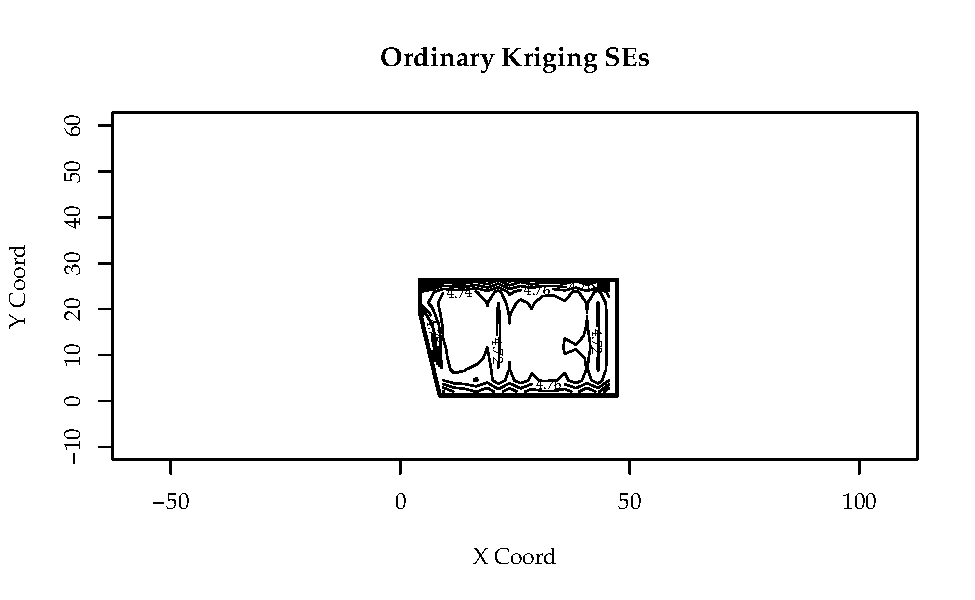
\includegraphics[width=\maxwidth]{figure/prob1d-4} 

}



\end{knitrout}


\end{enumerate}

\item

\begin{knitrout}\footnotesize
\definecolor{shadecolor}{rgb}{0.969, 0.969, 0.969}\color{fgcolor}\begin{kframe}
\begin{alltt}
\hlstd{C} \hlkwb{<-} \hlkwa{function}\hlstd{(}\hlkwc{t}\hlstd{)\{}
  \hlkwd{exp}\hlstd{(}\hlopt{-}\hlstd{(}\hlnum{3}\hlopt{*}\hlstd{t}\hlopt{/}\hlnum{5}\hlstd{))}
\hlstd{\}}

\hlstd{dist.dat} \hlkwb{<-} \hlkwd{dist}\hlstd{()}
\end{alltt}


{\ttfamily\noindent\bfseries\color{errorcolor}{Error in as.matrix(x): argument "{}x"{} is missing, with no default}}\end{kframe}
\end{knitrout}

\begin{knitrout}\footnotesize
\definecolor{shadecolor}{rgb}{0.969, 0.969, 0.969}\color{fgcolor}\begin{kframe}
\begin{alltt}
\hlstd{u}\hlkwb{<-}\hlkwd{seq}\hlstd{(}\hlnum{2}\hlstd{,}\hlnum{4}\hlstd{,}\hlkwc{l}\hlstd{=}\hlnum{1000}\hlstd{)}
\hlstd{m}\hlkwb{<-} \hlopt{-}\hlstd{(}\hlnum{1} \hlopt{-}\hlkwd{t}\hlstd{(one.vec)}\hlopt\hlkwd{solve}\hlstd{(Sigmat)}\hlopt\hlstd{sigvec.B)}\hlopt{/}\hlstd{(}
  \hlkwd{t}\hlstd{(one.vec)}\hlopt\hlkwd{solve}\hlstd{(Sigmat)}\hlopt\hlstd{one.vec)}
\end{alltt}


{\ttfamily\noindent\bfseries\color{errorcolor}{Error in t(one.vec): object 'one.vec' not found}}\begin{alltt}
\hlcom{# approximate sigma(B,B)}
\hlcom{# set up a storage vector which will contain the}
\hlcom{# point to block covariances between Z((2,4)) and}
\hlcom{# the individual points in the interval (2,4).}
\hlstd{e}\hlkwb{<-}\hlkwd{rep}\hlstd{(}\hlnum{0}\hlstd{,}\hlnum{1000}\hlstd{)}
\hlcom{# Now approximate the point to block covariances}
\hlcom{# Cov(Z(B),Z(u[i]) where u[i] is a point in B}
\hlkwa{for}\hlstd{(i} \hlkwa{in} \hlnum{1}\hlopt{:}\hlnum{1000}\hlstd{)\{}
 \hlstd{e[i]}\hlkwb{<-}\hlkwd{mean}\hlstd{(}\hlkwd{exp}\hlstd{(}\hlopt{-}\hlnum{3}\hlopt{*}\hlkwd{abs}\hlstd{(u}\hlopt{-}\hlstd{u[i])}\hlopt{/}\hlnum{5}\hlstd{))\}}
\hlcom{# now take the mean of all the point to block covariances}
\hlcom{# in e to get Cov(Z(B),Z(B))}
\hlstd{sig.BB}\hlkwb{<-}\hlkwd{mean}\hlstd{(e)}
\hlstd{sig.BB}
\end{alltt}
\begin{verbatim}
[1] 0.6958757
\end{verbatim}
\end{kframe}
\end{knitrout}

\end{enumerate}
\end{document}

